\chapter{Result and Evaluation}
\label{ResultandEvaluation}

Simulations are done respectively for both line and grid scenarios with different numbers of nodes (4, 9, 16) as well as different inter node distances (10 m, 50 m, 100 m). Furthermore, for each topology both OF0 and MRHOF are simulated. A hundred simulations are run for each scenario setup. Two simulation setups are used as examples in the evaluation: 9 nodes line scenario with 100 m inter node distance (will be referred as "the line scenario")  and 16 nodes grid scenario with 100 m inter node distance (will be referred as "the grid scenario"); more results of other topologies can be found in \ref{Simulation Results}All the results are the mean values of 100 runs. 

\section{Default Route Discovery Time}
\label{default route}

The default route discovery time is presented in the CDF manner. Figure \ref{fig:cdf} shows (TODO)
The initial interval size I is setted to  256 ms, according to the Trickle algorithm mentioned in Section \ref{Trickle}, the t is taken randomly from the interval [128, 256) ms. After booted, the root (node 1) multicasts its first DIO message in t ms once the Trickle timer is setted. Whichever node receives the message checks for the consistency between its own DODAG information and the ones DIO carries. Due to it is the first DIO it receives, the receiver decides the DIO contains information about a new DODAG. Then the receiver adds the default route through the root node (node 1), updates its information to join the DODAG, and sets its Trickle timer to the inital parameters. After Trickle timer fires, the receiver will send out its first DIO so the nodes which are more than one hop away from the root can add the default route though it.
\newline

\begin{figure}[htbp]
  \begin{center}
    \leavevmode
      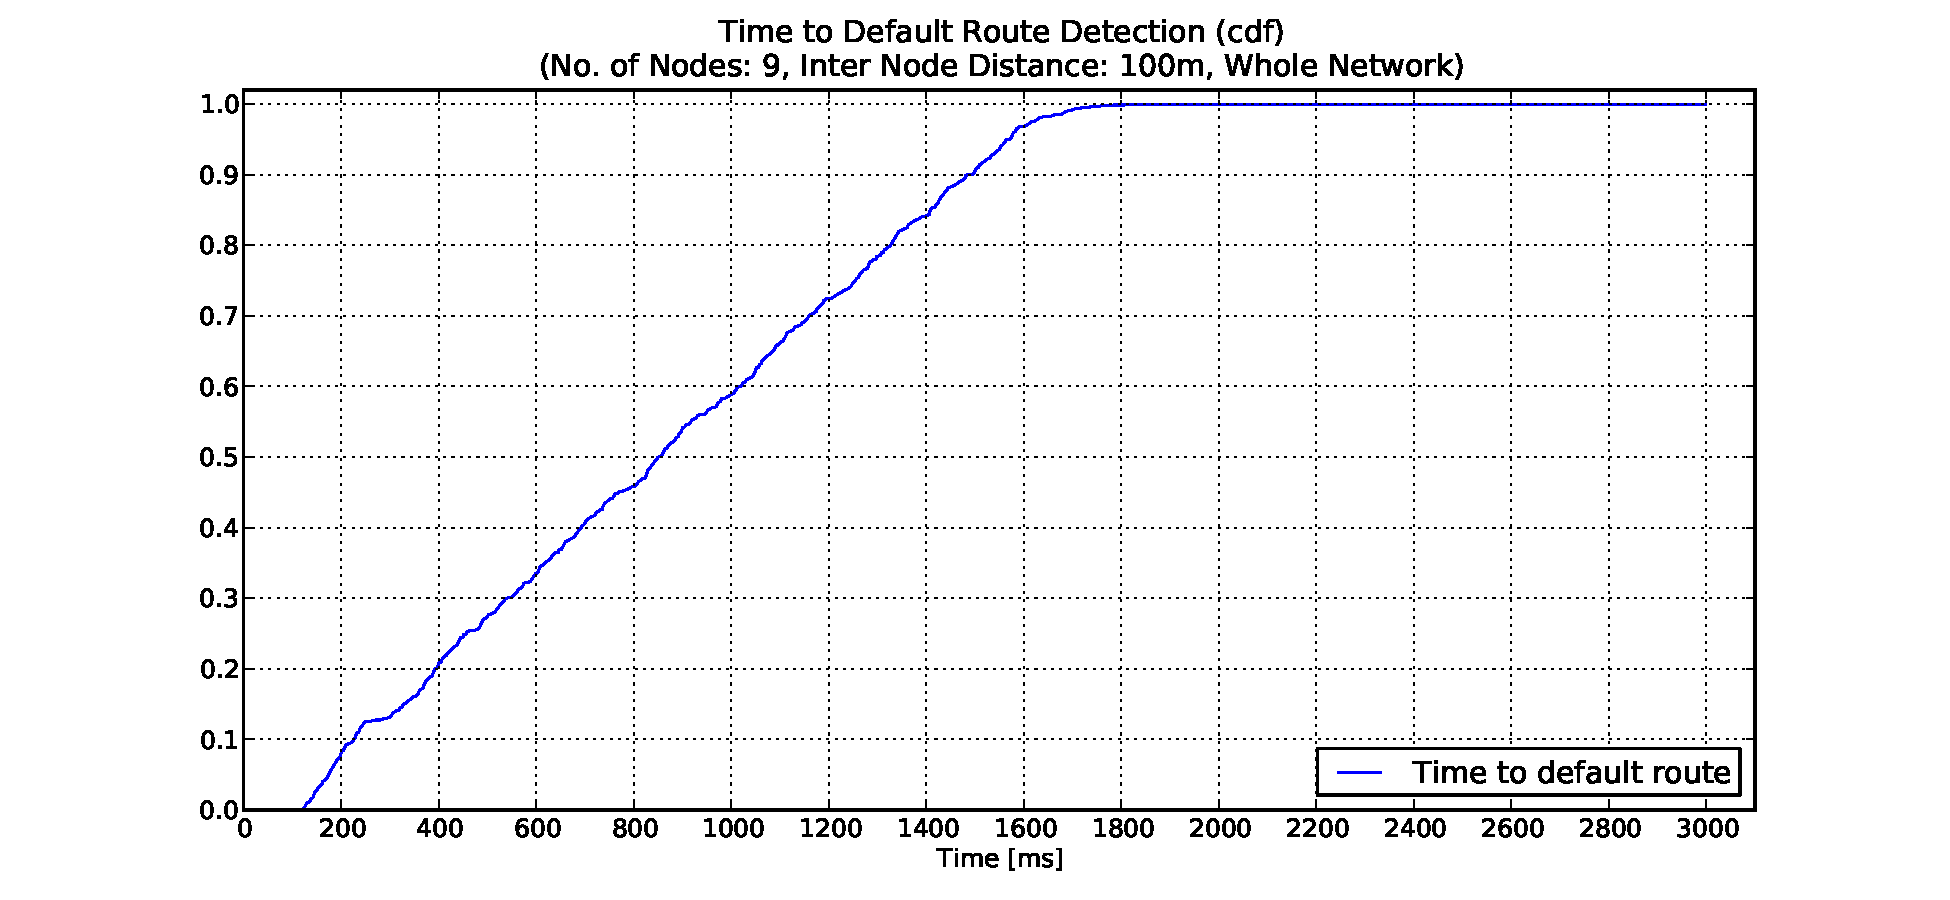
\includegraphics[scale=0.5]
      {/home/bo/Documents/Thesis/Final/Pics/results/9/MRHOF/grid/dist100_montecarlo_cdf_hist.pdf}
   \caption{CDF: the default route discovery time}
    \label{fig:cdf}
  \end{center}
\end{figure}

\section{Control Message Overhead}
\label{ICMP}
The main advantage of using Trickle algorithm is it reduces the number of control messages. Figure \ref{fig:icmp} shows the number of ICMP messages (DIS, DIO, DAO) for each node in two 10 minutes intervals. The time intervals are taken one after another and as soon as the nodes are booted. 
\begin{figure}[htbp]
  \begin{center}
    \leavevmode
    \subfloat[First 10 minutes]{\label{fig:icmp0}
      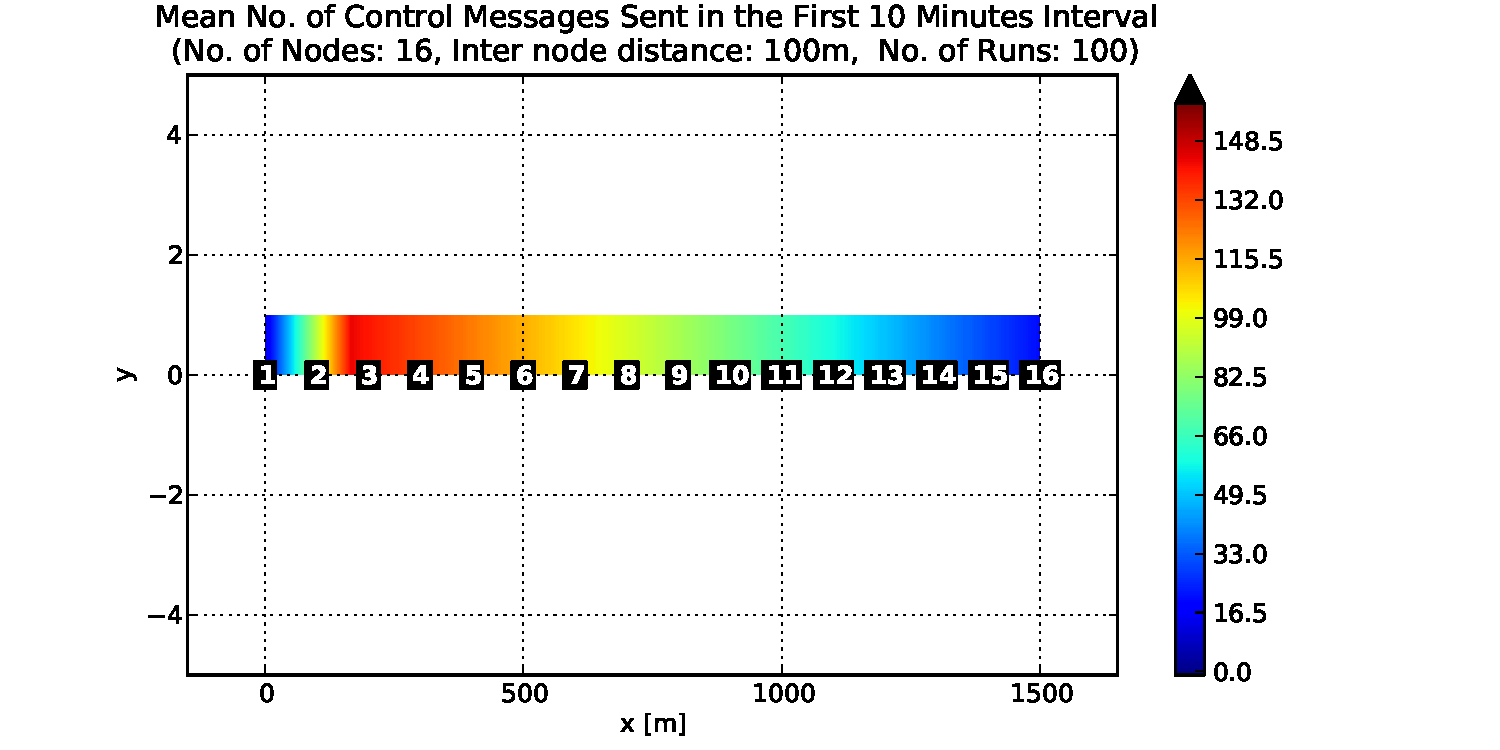
\includegraphics[scale=0.5]{/home/bo/Documents/Thesis/Final/Pics/results/9/MRHOF/grid/dist100_montecarlo_contour_sent_ICMP_0}}\\
    \subfloat[Second 10 minutes]{\label{fig:icmp1}
       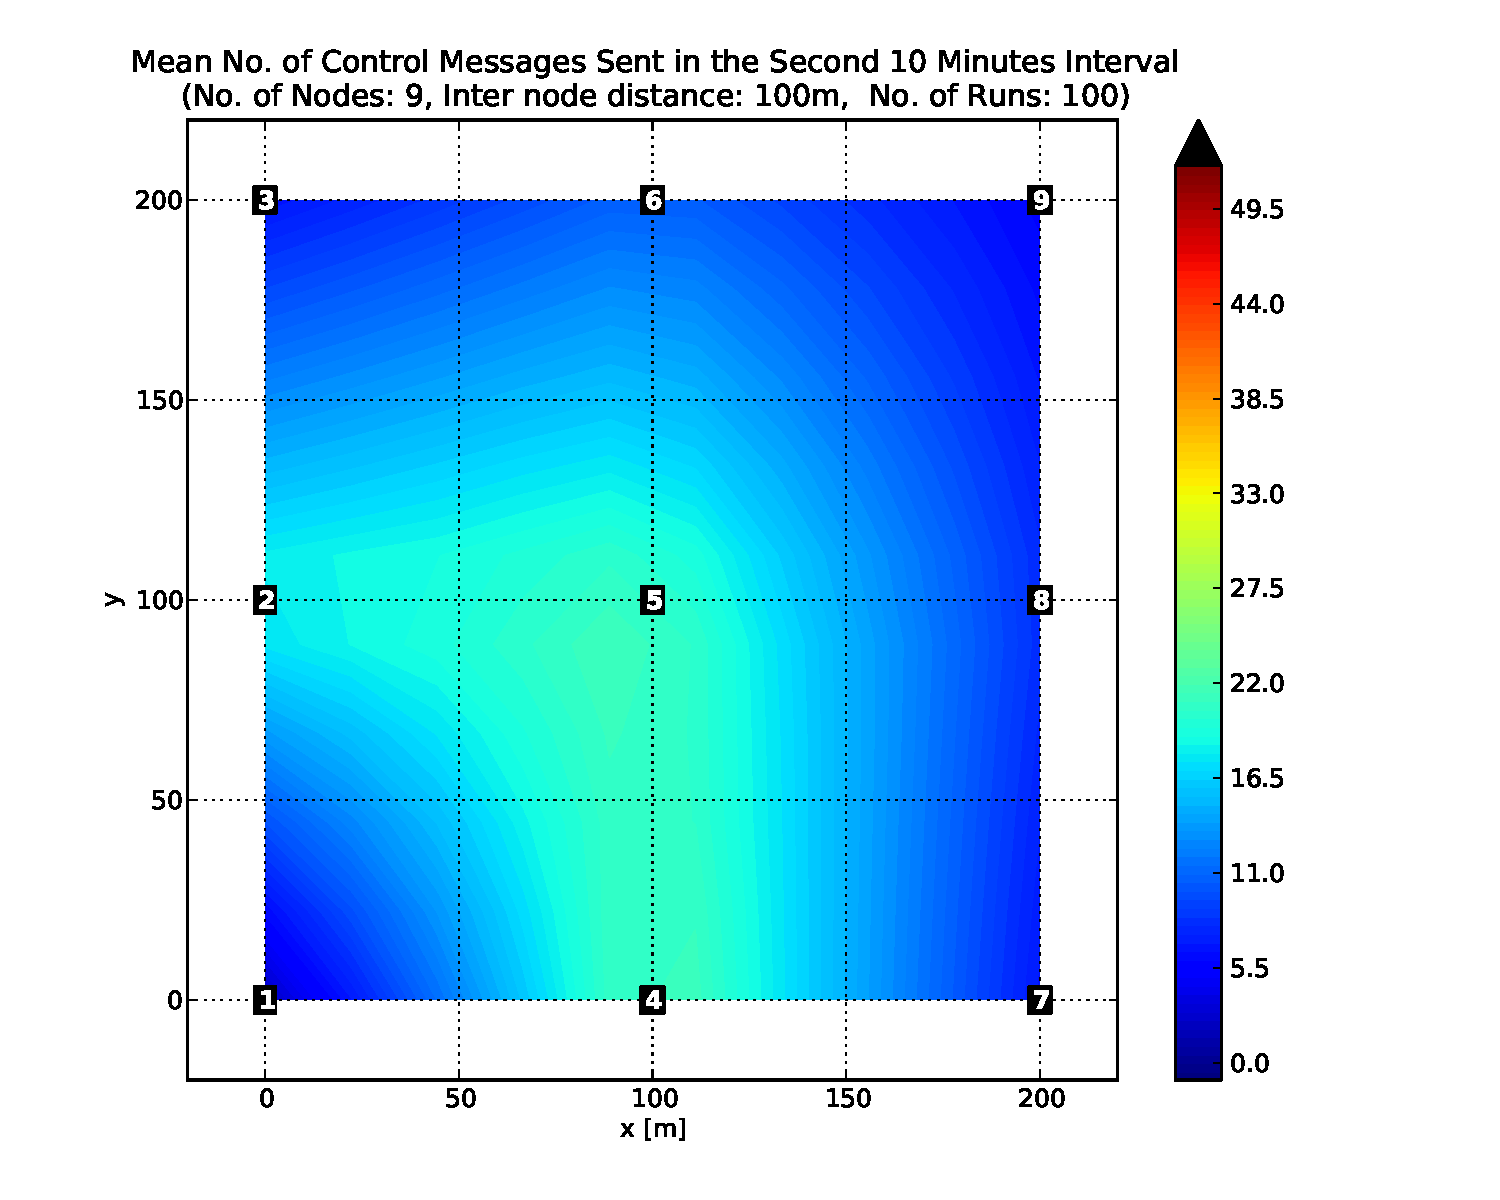
\includegraphics[scale=0.5]{/home/bo/Documents/Thesis/Final/Pics/results/9/MRHOF/grid/dist100_montecarlo_contour_sent_ICMP_1}}
    \caption{ICMP messages in a 9 nodes grid scenario with 100m inter node distance}
    \label{fig:icmp}
  \end{center}
\end{figure}
Node 1 sends the least ICMP messages in the first time interval (Figure \ref{fig:icmp0}) because as root it does not sent any DIS and DAO message. Another phenomenon can be observed - the lower rank (closer to the root) the node is, the more control messages it sends. The reason for that is (TODO)
\newline

In the second 10 minutes time interval the amount of control messages drops as the DODAG stabilizes due to the effect of Trickle timer.(TODO, a table shows how many exactly sent in first and second time interval)

\section{Packet Loss}
\label{PL}
\begin{figure}[htbp]
  \begin{center}
    \leavevmode
    \subfloat[OF0]{\label{fig:9_line_100_OF0_pl}
      \includegraphics[scale=0.5]{/home/bo/Documents/Thesis/Final/Pics/results/9/OF0/line/dist100_montecarlo_contour_packetloss.pdf}}\\
      %\vspace{20pt}
    \subfloat[MRHOF]{\label{fig:9_line_100_MRHOF_pl}
       \includegraphics[scale=0.5]{/home/bo/Documents/Thesis/Final/Pics/results/9/MRHOF/line/dist100_montecarlo_contour_packetloss.pdf}}
    \caption{Mean packet loss in a 16 nodes grid scenario wiht 100m inter node distance}
    \label{fig:9_line_100_pl}
  \end{center}
\end{figure}

\begin{figure}[htbp]
  \begin{center}
    \leavevmode
    \subfloat[OF0]{\label{fig:16_grid_100_OF0_pl}
      \includegraphics[scale=0.5]{/home/bo/Documents/Thesis/Final/Pics/results/16/OF0/grid/dist100_montecarlo_contour_packetloss.pdf}}\\
    \subfloat[MRHOF]{\label{fig:16_grid_100_MRHOF_pl}
       \includegraphics[scale=0.5]{/home/bo/Documents/Thesis/Final/Pics/results/16/MRHOF/grid/dist100_montecarlo_contour_packetloss.pdf}}
    \caption{Mean packet loss in a 16 nodes grid scenario wiht 100m inter node distance}
    \label{fig:16_grid_100_pl}
  \end{center}
\end{figure}

Packet loss rate of the two topologies for both OF0 and MRHOF are shown in Figure \ref{fig:9_line_100_pl} and Figure \ref{fig:16_grid_100_pl}. As the formulars presented in Section \ref{Sim:Scenarios}, the PRR will be 99.99\% received between two cloest nodes in both of the scenarios, and through multi-hop the packets are expected to be received properly by nodes that is more than one hop away.   
\newline 

For the line scenario, there is no difference between OF0 and MRHOF in packet loss rate. But for the grid scenario, OF0 is showing a packet loss around 15\%  on node 16 (the furthest to the root) while MRHOF still give almost no packet loss anywhere. This result shows that with OF0 a node is very likely to choose a routing parent with a unreliable link, such as a link with a low PRR. On the other hand, MRHOF with link ETX is guaranteed to choose the link with the least estimated transmission count, therefore the parent choosing mechanism is more stable and realiable. 

\section{Route Trip Time}
\label{RTT}

Mean Route Trip Time (RTT) of both OF0 and MRHOF are presented in Figure \ref{fig:rtt}. There is no difference between RTT results between OF0 and MRHOF again for the line scenario. The mean RTT  of each node for both topologies are presented in Table(TODO table)
\begin{figure}[htbp]
  \begin{center}
    \leavevmode
    \subfloat[OF0]{\label{fig:OF0_rtt}
      \includegraphics[scale=0.5]{/home/bo/Documents/Thesis/Final/Pics/results/16/OF0/grid/dist100_montecarlo_contour.pdf}}\\
    \subfloat[MRHOF]{\label{fig:MRHOF_rtt}
       \includegraphics[scale=0.5]{/home/bo/Documents/Thesis/Final/Pics/results/16/MRHOF/grid/dist100_montecarlo_contour.pdf}}
    \caption{Mean RTT in a 16 nodes grid scenario wiht 100m inter node distance}
    \label{fig:rtt}
  \end{center}
\end{figure} 




